%!TEX root = ../RelazioneStrutturaleMeoliNicola.tex
\begin{figure}[tbp]
\centering
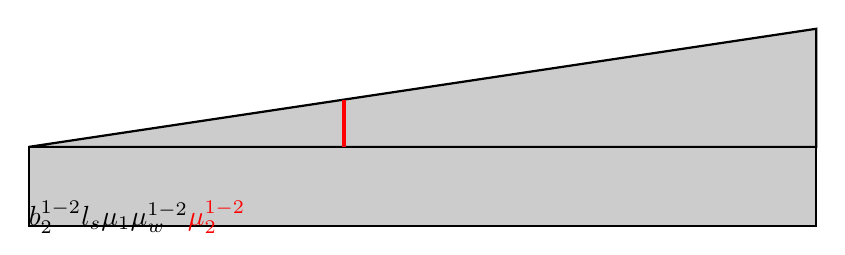
\begin{tikzpicture}
\draw[fill=black!20,thick] (0,0) rectangle (10,1);
\draw[fill=black!20,thick] (0,1) -- (10,1) -- (10,2.5) -- cycle;
\draw[red,ultra thick] (4,1) -- (4,1.6);
\dimensioning{1}{4,0}{10,0}{-.7}[$b_2^{1-2}$];
\dimensioning{1}{0,0}{10,0}{-1.4}[$l_s$];
\dimensioning{2}{10,0}{10,1}{10.7}[$\mu_1$];
\dimensioning{2}{10,0}{10,2.5}{11.4}[$\mu_w^{1-2}$];
\begin{scope}[color=red]
\dimensioning{2}{10,0}{10,1.6}{12.1}[$\mu_2^{1-2}$];
\end{scope}
\end{tikzpicture}
\caption{Coefficiente $\mu_2$ calcolato tramite somma dell'altezza del triangolo (ottenuta per similitudine rispetto la base) e il coefficiente $\mu_1$}
\label{fig:TriangoliSimiliNeve}
\end{figure}